% bubble sort example with a simple input: 3 1 4 2

\documentclass[beamer]{standalone}

\usepackage{ifthen}
\usepackage{tikz}
\usetikzlibrary{arrows.meta, fit, backgrounds}

\begin{document}

\begin{frame}{Bubble Sort Example}
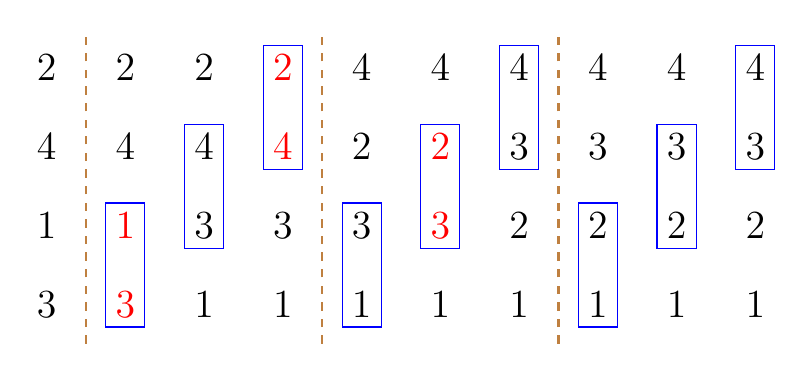
\begin{tikzpicture}[rotate = 90, swap/.style = {dashed, thick},
	inv/.style = {blue, rectangle, draw, inner sep = 0pt, outer sep = 0pt},
	ele/.style = {font = \Large},
	pass/.style = {brown, thick, dashed}]
	\uncover<1->{
  \foreach \e [count = \ei] in {3,1,4,2} {
	  \node (1\e) [ele] at (\ei, 1) {$\e$};
  }
  \draw [pass] (0.5, 0.5) to (4.5,0.5);
}

\uncover<2->{
  \foreach \e [count = \ei] in {3,1,4,2} {
	  \node (1\e) [ele] at (\ei, 0) {\ifthenelse{\e = 3 \OR \e = 1}{\textcolor{red}{$\e$}}{$\e$}};
  }
  \begin{pgfonlayer}{background}
    \node<2-> () [inv, fit = (13) (11)] {};
  \end{pgfonlayer}
}

\uncover<3->{
  \foreach \e [count = \ei] in {1,3,4,2} {
    \node (2\e) [ele] at (\ei, -1) {$\e$};
  }
  \begin{pgfonlayer}{background}
    \node<3-> () [inv, fit = (23) (24)] {};
  \end{pgfonlayer}
}

\uncover<4->{
  \foreach \e [count = \ei] in {1,3,4,2} {
	  \node (3\e) [ele] at (\ei, -2) {\ifthenelse{\e = 4 \OR \e = 2}{\textcolor{red}{$\e$}}{$\e$}};
  }
  \begin{pgfonlayer}{background}
    \node<4-> () [inv, fit = (34) (32)] {};
  \end{pgfonlayer}
  % the second pass
  \draw [pass] (0.5, -2.5) to (4.5,-2.5);
}

\uncover<5->{
  \foreach \e [count = \ei] in {1,3,2,4} {
	  \node (4\e) [ele] at (\ei, -3) {$\e$};
  }
  \begin{pgfonlayer}{background}
    \node<5-> () [inv, fit = (41) (43)] {};
  \end{pgfonlayer}
}

\uncover<6->{
  \foreach \e [count = \ei] in {1,3,2,4} {
	  \node (5\e) [ele] at (\ei, -4) {\ifthenelse{\e = 3 \OR \e = 2}{\textcolor{red}{$\e$}}{$\e$}};
  }
  \begin{pgfonlayer}{background}
    \node<6-> () [inv, fit = (53) (52)] {};
  \end{pgfonlayer}
}

\uncover<7->{
  \foreach \e [count = \ei] in {1,2,3,4} {
	  \node (6\e) [ele] at (\ei, -5) {$\e$};
  }
  \begin{pgfonlayer}{background}
    \node<7-> () [inv, fit = (63) (64)] {};
  \end{pgfonlayer}

  \draw [pass] (0.5, -5.5) to (4.5,-5.5);
}

\uncover<8->{
  \foreach \e [count = \ei] in {1,2,3,4} {
	  \node (7\e) [ele] at (\ei, -6) {$\e$};
  }
  \begin{pgfonlayer}{background}
    \node<8-> () [inv, fit = (71) (72)] {};
  \end{pgfonlayer}
}

\uncover<9->{
  \foreach \e [count = \ei] in {1,2,3,4} {
	  \node (8\e) [ele] at (\ei, -7) {$\e$};
  }
  \begin{pgfonlayer}{background}
    \node<9-> () [inv, fit = (82) (83)] {};
  \end{pgfonlayer}
}

\uncover<10->{
  \foreach \e [count = \ei] in {1,2,3,4} {
	  \node (9\e) [ele] at (\ei, -8) {$\e$};
  }
  \begin{pgfonlayer}{background}
    \node<10-> () [inv, fit = (93) (94)] {};
  \end{pgfonlayer}
}
\end{tikzpicture}
\end{frame}
\end{document}
